% ============================================================
% HygieneBench — IEEE Conference Paper
% Target venue: ACM CCS AISec Workshop (or IEEE S&P Workshop)
% Class: IEEEtran (conference mode)
%
% To compile:
%   pdflatex main.tex
%   bibtex main
%   pdflatex main.tex
%   pdflatex main.tex
%
% Download IEEEtran.cls from:
%   https://www.ieee.org/conferences/publishing/templates.html
% ============================================================

\documentclass[conference]{IEEEtran}

% ---- Packages -------------------------------------------------------
\usepackage[T1]{fontenc}
\usepackage[utf8]{inputenc}
\usepackage{cite}
\usepackage{amsmath,amssymb}
\usepackage{graphicx}
\usepackage{booktabs}
\usepackage{multirow}
\usepackage{array}
\usepackage{url}
\usepackage{hyperref}
\usepackage{xspace}
\usepackage{enumitem}
\usepackage{microtype}
\usepackage{balance}
\usepackage{tikz}
\usetikzlibrary{shapes.geometric, arrows.meta, positioning, fit, backgrounds, calc}

% ---- Macros ---------------------------------------------------------
\newcommand{\hb}{\textsc{HygieneBench}\xspace}
\newcommand{\fp}{$\blacktriangleright$\xspace}   % failure flag

% ---- TikZ styles ----------------------------------------------------
\tikzset{
  box/.style={rectangle, rounded corners=3pt, draw, thick,
              align=center, minimum height=1.6em, font=\small},
  bluebox/.style={box, fill=blue!12, draw=blue!50},
  greenbox/.style={box, fill=green!12, draw=green!50},
  orangebox/.style={box, fill=orange!12, draw=orange!50},
  redbox/.style={box, fill=red!10, draw=red!40},
  graybox/.style={box, fill=gray!10, draw=gray!40},
  arrow/.style={-Stealth, thick},
  groupfit/.style={draw=gray!50, dashed, rounded corners=4pt, inner sep=4pt},
}

% =====================================================================
\begin{document}

\title{HygieneBench: A Reproducible Synthetic Benchmark\\
       for Cyber-Hygiene Anomaly Detection\\
       Across Identity, Endpoint, and Patch Telemetry}

\author{
  \IEEEauthorblockN{Harshavardhan Malla}
  \IEEEauthorblockA{Independent Researcher}
}

\maketitle

% ---- Abstract -------------------------------------------------------
\begin{abstract}
Cyber-hygiene anomaly detection---identifying stale privileged accounts,
dormant-account reactivations, endpoint-agent coverage gaps, patch noncompliance
clusters, and telemetry missingness---is operationally important but poorly served
by existing public benchmarks, which focus predominantly on network intrusion or
attack-emulation telemetry. We introduce \hb, an open, reproducible benchmark that
jointly covers Active Directory identity state, endpoint patch posture,
vulnerability exposure, and telemetry freshness across seven evaluation tasks
(T1--T7) and twelve anomaly classes. All telemetry is generated from a seeded
synthetic pipeline grounded in public structural priors (NIST NVD severity
distributions, Verizon DBIR 2026 patch-lag aggregates, CISA BOD 23-01
cadence requirements). We evaluate eight detection methods under five telemetry
conditions (baseline, fresh, stale, missing, unsupervised) across 810 runs using a
pre-registered failure protocol. Our central finding is that \textbf{86.2\% of
(condition, task, method) configurations fail to consistently outperform a
structured rule baseline} by the pre-registered \(\Delta\!\geq\!0.05\) AP
threshold. ML adds meaningful signal on group-membership-drift detection (T2, best
ML: temporal z-score, \(+\)0.185 AP) and patch-vulnerability hygiene (T5, best ML:
OCSVM, \(+\)0.210 AP). Generator, datasets, and evaluation harness are openly
released.
\end{abstract}

\begin{IEEEkeywords}
cyber hygiene, anomaly detection, benchmark, synthetic data, Active Directory,
endpoint security, negative-result reporting
\end{IEEEkeywords}

% =====================================================================
\section{Introduction}
\label{sec:intro}

Security operations centers (SOCs) in public-sector environments face persistent
cyber-hygiene failures: stale privileged accounts invisible to behavioral analytics,
endpoints lacking agent coverage, unpatched vulnerabilities aged well beyond CISA
Binding Operational Directive 23-01 deadlines \cite{cisa_bod2301_2022}, and
telemetry gaps that silently degrade detection confidence. NIST SP 800-40 Rev.\ 4
\cite{nist_sp800_40} frames enterprise patch management as a risk-based discipline
requiring current, accurate asset and patch telemetry. Hygiene-state monitoring
is a prerequisite for downstream identity and endpoint detection---without knowing
which accounts are dormant, which agents are missing, and which patches are overdue,
higher-order anomalies cannot be reliably attributed.

Yet no public benchmark exists for this problem class. Existing collections---the
LANL Unified Host and Network Dataset \cite{kent2015lanl}, the CERT Insider Threat
Dataset \cite{glasser2013cert}, CICIDS \cite{sharafaldin2018cicids}, and
attack-emulation repositories \cite{rodriguez2019mordor}---provide rich telemetry
for network intrusion or insider-threat detection but do not model identity hygiene
state, patch posture, vulnerability exposure, or telemetry freshness as first-class
evaluation axes.

This paper makes the following contributions:
\begin{itemize}[leftmargin=*,noitemsep,topsep=2pt]
  \item[\textbf{C1}] A fully open, seeded synthetic telemetry generator covering
    eleven entity/event tables with documented structural priors.
  \item[\textbf{C2}] A twelve-class cyber-hygiene anomaly taxonomy with
    ATT\&CK enabling-condition mappings.
  \item[\textbf{C3}] Seven benchmark evaluation tasks under five telemetry
    conditions with pre-registered evaluation budgets.
  \item[\textbf{C4}] An 810-run comparative evaluation of eight detection methods
    with a pre-registered failure protocol.
  \item[\textbf{C5}] Explicit negative-result reporting for 86.2\% of
    configurations, with analysis of when and why ML fails to add value.
\end{itemize}

% =====================================================================
\section{Related Work}
\label{sec:related}

\textbf{Intrusion and attack-emulation benchmarks.}
LANL \cite{kent2015lanl}, CICIDS \cite{sharafaldin2018cicids}, and DARPA TC
\cite{darpa_tc_2018} target network-level events. Mordor/Security Datasets
\cite{rodriguez2019mordor} provides attack-emulation telemetry from red-team
exercises. None models hygiene state or telemetry freshness as controlled
evaluation variables.

\textbf{Insider threat datasets.}
The CERT dataset \cite{glasser2013cert} covers user behavior for insider-threat
detection but does not include patch posture, vulnerability records, or the
multi-table structure characteristic of enterprise AD environments.

\textbf{Graph anomaly detection.}
Attributed-graph anomaly detection has produced several methods and datasets,
including DOMINANT \cite{ding2019dominant} and PyGOD \cite{liu2024pygod}, which
operate on single-hop graph structure and do not model the temporal, multi-table
telemetry of enterprise security operations.

\textbf{Synthetic generation.}
Synthetic dataset generation has precedent in network simulation
\cite{creech2013kdd}. \hb extends this tradition to the hygiene-state domain with
eleven entity/event tables and publicly citable structural priors (NIST SP
800-40 \cite{nist_sp800_40}, CISA BOD 23-01 \cite{cisa_bod2301_2022}).

\textbf{Negative-result reporting.}
Explicitly reporting when ML fails to outperform simpler baselines is established
in machine learning \cite{sculley2018winners} but underrepresented in security
benchmarks. \hb operationalizes this with a pre-registered
$\Delta$-threshold protocol.

% =====================================================================
\section{\hb Design}
\label{sec:design}

\subsection{System Architecture}

Fig.~\ref{fig:architecture} shows the \hb pipeline. A seeded generator produces
eleven entity/event tables under configurable telemetry conditions. An anomaly
injector marks ground-truth labels across twelve anomaly classes. A deterministic
splitter partitions entities into train/val/test splits. The evaluation harness
extracts task-specific features, fits eight detection methods, and applies the
pre-registered failure protocol to produce primary results and failure flags.

% ---- Architecture TikZ Diagram --------------------------------------
\begin{figure}[t]
\centering
\scalebox{0.78}{%
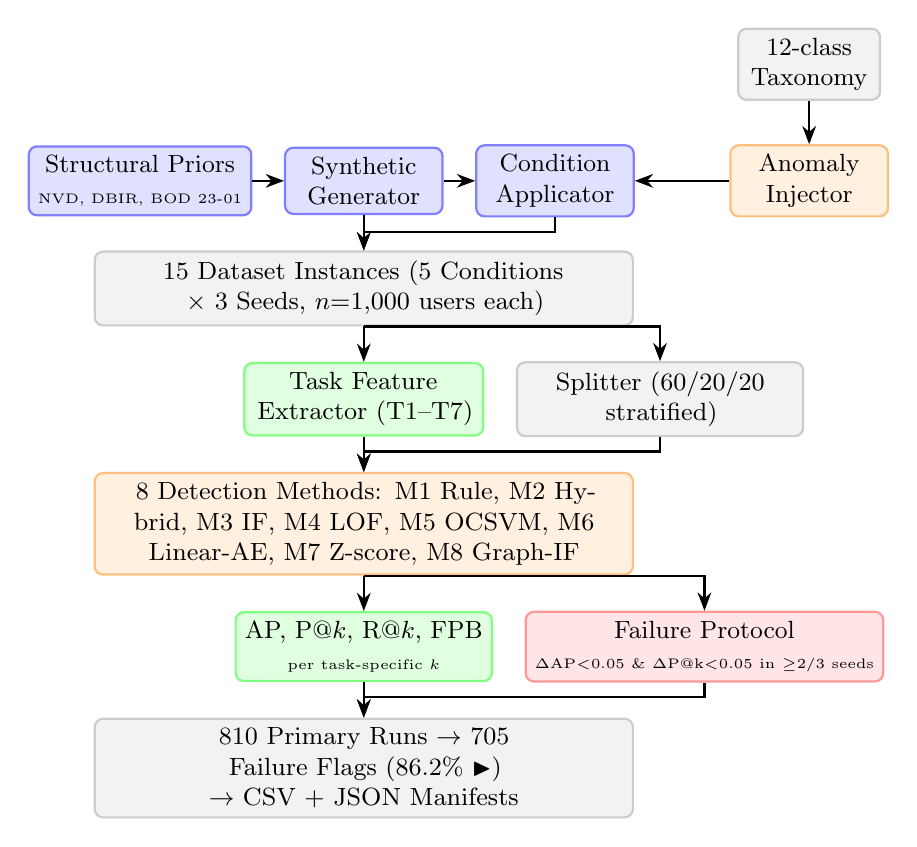
\begin{tikzpicture}[node distance=0.55cm and 0.4cm]

  % Row 1: Data generation
  \node[bluebox, minimum width=2.2cm] (priors)
    {Structural Priors\\{\tiny NVD, DBIR, BOD 23-01}};
  \node[bluebox, minimum width=2.0cm, right=of priors] (gen)
    {Synthetic\\Generator};
  \node[bluebox, minimum width=2.0cm, right=of gen] (cond)
    {Condition\\Applicator};

  % Row 1 arrows
  \draw[arrow] (priors) -- (gen);
  \draw[arrow] (gen) -- (cond);

  % Row 2: Datasets
  \node[graybox, minimum width=6.8cm, text width=6.6cm, below=0.45cm of gen] (datasets)
    {15 Dataset Instances (5 Conditions $\times$ 3 Seeds, $n$=1,000 users each)};

  \draw[arrow] (cond.south) -- ++(0,-0.18) -| (datasets.north);
  \draw[arrow] (gen.south)  -- ++(0,-0.18) -| (datasets.north);

  % Injector node - to the right
  \node[orangebox, minimum width=2.0cm, right=1.2cm of cond] (inj)
    {Anomaly\\Injector};
  \draw[arrow] (inj.west) -- (cond.east);
  \node[graybox, minimum width=1.8cm, above=0.55cm of inj] (tax)
    {12-class\\Taxonomy};
  \draw[arrow] (tax) -- (inj);

  % Row 3: Feature Extraction
  \node[greenbox, minimum width=3.0cm, text width=2.8cm, below=0.45cm of datasets] (feat)
    {Task Feature Extractor (T1--T7)};
  \node[graybox, minimum width=3.6cm, text width=3.4cm, right=0.4cm of feat] (split)
    {Splitter (60/20/20 stratified)};

  \draw[arrow] (datasets.south) -| (feat.north);
  \draw[arrow] (datasets.south) -| (split.north);

  % Row 4: Methods
  \node[orangebox, minimum width=6.8cm, text width=6.6cm, below=0.45cm of feat] (methods)
    {8 Detection Methods: M1 Rule, M2 Hybrid, M3 IF, M4 LOF, M5 OCSVM,
     M6 Linear-AE, M7 Z-score, M8 Graph-IF};

  \draw[arrow] (feat.south) -- ++(0,-0.18) -| (methods.north);
  \draw[arrow] (split.south) -- ++(0,-0.18) -| (methods.north);

  % Row 5: Metrics + Failure Protocol
  \node[greenbox, minimum width=3.2cm, below=0.45cm of methods] (metrics)
    {AP, P@$k$, R@$k$, FPB\\{\tiny per task-specific $k$}};
  \node[redbox, minimum width=3.4cm, right=0.4cm of metrics] (fail)
    {Failure Protocol\\{\tiny $\Delta$AP$<$0.05 \& $\Delta$P@k$<$0.05 in $\geq$2/3 seeds}};

  \draw[arrow] (methods.south) -| (metrics.north);
  \draw[arrow] (methods.south) -| (fail.north);

  % Row 6: Results
  \node[graybox, minimum width=6.8cm, text width=6.6cm, below=0.45cm of metrics] (results)
    {810 Primary Runs $\rightarrow$ 705 Failure Flags (86.2\% \fp)\\$\rightarrow$ CSV + JSON Manifests};

  \draw[arrow] (metrics.south) -- ++(0,-0.18) -| (results.north);
  \draw[arrow] (fail.south)    -- ++(0,-0.18) -| (results.north);

\end{tikzpicture}%
}% end \scalebox
\caption{\hb end-to-end pipeline. Shaded boxes indicate the generator/condition
  layer (blue), evaluation harness (green), injector (orange), and outputs (gray/red).}
\label{fig:architecture}
\end{figure}
% ---- End Diagram ----------------------------------------------------

\subsection{Schema and Generator}

\hb v0.1 generates eleven entity/event tables and one anomaly label table
(Table~\ref{tab:schema}). The generator uses \texttt{numpy.random.default\_rng(seed)}
for all randomness; entity IDs are deterministic UUIDs from
\texttt{hashlib.md5(seed\_tag + index)}.

\begin{table}[t]
\centering
\caption{\hb v0.1 schema (medium scale, $n$=1,000 users)}
\label{tab:schema}
\footnotesize
\setlength{\tabcolsep}{3pt}
\begin{tabular}{@{} >{\ttfamily\raggedright\arraybackslash}p{4.5cm}
                    r
                    >{\raggedright\arraybackslash}p{2.5cm} @{}}
\toprule
\normalfont Table & Rows & Description \\
\midrule
users                     & 1,000      & AD user accounts, identity state \\
groups                    & 65         & AD security/distribution groups \\
computers                 & 830        & Managed endpoints \\
assets                    & 830        & Asset inventory entries \\
login\_events             & $\sim$249k & Authentication events (30 days) \\
group\_membership\_events & $\sim$51   & Group add/remove events \\
account\_lifecycle\_events & varies    & Account create/disable/enable \\
endpoint\_patch\_state    & 830        & Patch compliance snapshot \\
vulnerability\_records    & $\sim$3.5k & Per-endpoint CVE exposures \\
remediation\_events       & varies     & Patch/remediation actions \\
telemetry\_freshness\_log & varies     & Per-entity source freshness \\
anomaly\_labels           & 110        & Ground truth (task + split) \\
\bottomrule
\end{tabular}
\end{table}

\textbf{Structural priors.} Patch-lag distributions follow DBIR 2026 aggregate
statistics (43-day mean for critical patches). CVE severity distributions follow
NVD base score bins. Telemetry cadence thresholds follow CISA BOD 23-01 (14-day
asset discovery, 72-hour patch data) \cite{cisa_bod2301_2022}. AD group-size
distributions have no peer-reviewed source and are modeled via disclosed
assumptions (power-law approximation) documented in the dataset card.

\textbf{Conditions.} Five parameterized conditions isolate the effect of telemetry
quality on detection: \textbf{C-BASE} (no staleness); \textbf{C-FRESH} (elevated
freshness flagging); \textbf{C-STALE} (20\% of entities have $>$14-day telemetry
gaps); \textbf{C-MISS} (one data source absent for 15\% of entities);
\textbf{C-UNSUP} (C-BASE with anomaly labels withheld from training). Each
condition is generated for seeds 42, 137, and 2024, yielding 15 dataset instances.

\subsection{Anomaly Taxonomy}

Table~\ref{tab:taxonomy} lists the twelve anomaly classes with ATT\&CK
enabling-condition mappings. These mappings denote correlated enabling conditions,
not detection claims for specific techniques.

\begin{table}[t]
\centering
\caption{Cyber-hygiene anomaly taxonomy. ATT\&CK mappings are enabling-condition
  correlations only.}
\label{tab:taxonomy}
\scriptsize
\begin{tabular}{@{}llll@{}}
\toprule
Code & Class & ATT\&CK enabling condition & Task(s) \\
\midrule
AH-01 & Stale privileged account       & Valid Accounts (T1078.002)    & T1 \\
AH-02 & Privilege escalation drift     & Domain Policy Modification    & T7 \\
AH-03 & Group membership drift         & Domain Policy Mod. (T1484)    & T2 \\
AH-04 & Dormant account reactivation   & Valid Accounts (T1078.002)    & T6 \\
AH-05 & Impossible/unusual login       & Lateral Movement enabling     & T1,T3 \\
AH-06 & Endpoint--identity risk corr.  & Initial Access enabling       & T3 \\
AH-07 & Patch noncompliance cluster    & Exploit Public-Facing (T1190) & T5 \\
AH-08 & KEV exposure aging             & Exploit Public-Facing (T1190) & T5 \\
AH-09 & Asset inventory mismatch       & Defense Evasion enabling      & T4 \\
AH-10 & Missing endpoint agent         & Defense Evasion enabling      & T4 \\
AH-11 & Telemetry missingness cluster  & Defense Evasion enabling      & T4 \\
AH-12 & Abnormal remediation delay     & Exploit Public-Facing         & T5 \\
\bottomrule
\end{tabular}
\end{table}

\subsection{Benchmark Tasks}

Seven tasks cover the twelve anomaly classes across different entity scopes and
temporal windows (Table~\ref{tab:tasks}). The $k$ values in Table~\ref{tab:tasks}
are pre-registered per TASK\_SPECS.md and reflect operational SOC daily review
budgets, not post-hoc tuning.

\begin{table}[t]
\centering
\caption{Benchmark tasks. Imbalance ratios are per dataset instance ($n$=1,000).}
\label{tab:tasks}
\scriptsize
\begin{tabular}{@{}lllrr@{}}
\toprule
Task & Description & Scope & $k$ & Imbalance \\
\midrule
T1 & Stale privileged account risk      & Priv. users        & 10 & 1:50  \\
T2 & Group membership drift             & Users w/ grp events & 20 & 1:167 \\
T3 & Endpoint--identity risk correlation & Users w/ endpoints  & 15 & 1:333 \\
T4 & Telemetry coverage gaps            & All computers/assets & 20 & 1:14  \\
T5 & Patch--vulnerability hygiene       & All computers       & 25 & 1:59  \\
T6 & Dormant account reactivation       & Users w/ lifecycle  & 10 & 1:250 \\
T7 & Escalation drift detection         & Users w/ grp adds   & 10 & 1:500 \\
\bottomrule
\end{tabular}
\end{table}

% =====================================================================
\section{Experimental Setup}
\label{sec:setup}

\subsection{Detection Methods}

Table~\ref{tab:methods} describes the eight methods. All methods are applied to
pre-computed task feature matrices; missing values are imputed with training-set
column means. M8 is excluded from T4 and T5 by design (no meaningful graph signal
for asset/patch anomalies).

\begin{table}[t]
\centering
\caption{Detection methods evaluated in \hb}
\label{tab:methods}
\scriptsize
\begin{tabular}{@{}lll>{\raggedright\arraybackslash}p{3.0cm}@{}}
\toprule
ID & Name & Type & Notes \\
\midrule
M1 & Rule baseline  & Task rules       & Per-task thresholds; no training \\
M2 & Hybrid scorer  & Weighted sum     & Identity + endpoint + vuln + freshness \\
M3 & Isolation Forest & Ensemble       & 200 trees, contamination=0.02 \\
M4 & LOF            & Density          & $k$=20, novelty mode, MinMaxScaler \\
M5 & OCSVM          & Kernel           & $\nu$=0.05, RBF, MinMaxScaler \\
M6 & Linear-AE      & Reconstruction   & PCA-based (dim=8); linear AE approx. \\
M7 & Temporal z-score & Statistical    & Population z-score on task features \\
M8 & Graph-IF       & Graph+ensemble   & Bipartite networkx + IF; DOMINANT approx. \cite{ding2019dominant} \\
\bottomrule
\end{tabular}
\end{table}

\subsection{Feature Engineering}

For each task, a deterministic feature extractor computes a flat tabular feature
matrix from the eleven raw CSV tables. Features are task-scoped: only columns
relevant to the task entity type and anomaly class are included.
Table~\ref{tab:features} lists the primary feature groups per task.

\begin{table}[t]
\centering
\caption{Primary task features (3--5 per task). All features computed from raw
  tables; no features constructed post-hoc.}
\label{tab:features}
\scriptsize
\begin{tabular}{@{} l >{\raggedright\arraybackslash}p{5.8cm} @{}}
\toprule
Task & Key features \\
\midrule
T1 & \texttt{days\_since\_last\_logon}, \texttt{privileged\_group\_count},
     \texttt{is\_service\_account}, \texttt{source\_freshness\_flag} \\
T2 & \texttt{group\_change\_count\_30d}, \texttt{priv\_group\_change\_count\_30d},
     \texttt{priv\_add\_ratio}, \texttt{actor\_diversity} \\
T3 & \texttt{is\_privileged}, \texttt{days\_since\_agent\_heartbeat},
     \texttt{patch\_compliance\_score}, \texttt{open\_kev\_count},
     \texttt{network\_segment\_risk} \\
T4 & \texttt{endpoint\_agent\_installed}, \texttt{inventory\_mismatch\_flag},
     \texttt{days\_since\_heartbeat}, \texttt{freshness\_gap\_days} \\
T5 & \texttt{patch\_compliance\_score}, \texttt{critical\_missing\_patch\_count},
     \texttt{open\_kev\_count}, \texttt{max\_kev\_days\_open},
     \texttt{remediation\_latency\_mean} \\
T6 & \texttt{dormant\_days\_at\_reactivation}, \texttt{off\_hours\_rate},
     \texttt{cross\_segment\_rate}, \texttt{is\_privileged} \\
T7 & \texttt{priv\_adds\_30d}, \texttt{priv\_add\_rate},
     \texttt{group\_change\_velocity}, \texttt{actor\_count} \\
\bottomrule
\end{tabular}
\end{table}

Missing values (arising under C-MISS) are imputed with training-set column means
before fitting. All features are computed identically for every method; no
method-specific feature selection or preprocessing is applied beyond MinMaxScaler
where noted in Table~\ref{tab:methods}.

\subsection{Metrics and Failure Protocol}

\textbf{Primary:} Average Precision (AP) and Precision@$k$ (P@$k$) at the
task-specific $k$ values in Table~\ref{tab:tasks}. \textbf{Secondary:} Recall@$k$,
False Positive Burden (FPB = 1$-$P@$k$), and AP rank stability (1$-$CV across
seeds).

\textbf{Pre-registered failure protocol.} A (condition, task, method) triple is
flagged as a \emph{negative result} (\fp) when:
\begin{align}
  &\mathrm{AP}_\mathrm{method} - \mathrm{AP}_\mathrm{rule} < 0.05 \notag \\
  &\quad\text{AND}\quad
  \mathrm{P@}k_\mathrm{method} - \mathrm{P@}k_\mathrm{rule} < 0.05
  \label{eq:failure}
\end{align}
in at least $\lceil\frac{2}{3} \times 3\rceil = 2$ of 3 seeds. M1 (rule) is
the reference; it is not flagged. The protocol was locked in the project decision
log prior to any results being examined.

% =====================================================================
\section{Results}
\label{sec:results}

\subsection{Overall Performance}

Table~\ref{tab:overall} summarizes performance across all 810 runs.
\textbf{608 of 705 (condition, task, method) configurations are failure-flagged
(86.2\%).} The rule baseline (M1) achieves the highest mean AP (0.916). M5 (OCSVM)
is the strongest ML method (AP~=~0.913, failure rate~69.5\%). M8 (graph) is
failure-flagged on every configuration (100\%).

\begin{table}[t]
\centering
\caption{Mean AP and P@$k$ across all 810 runs. \fp\ = failure-flagged.
  $\dagger$M8 covers T1--T3,T6--T7 only ($n$=75 configs).}
\label{tab:overall}
\small
\begin{tabular}{@{}lrrl@{}}
\toprule
Method & AP & P@$k$ & Failure rate \\
\midrule
M1 Rule baseline    & \textbf{0.916} & 0.444 & --- \\
M5 OCSVM            & 0.913 & \textbf{0.447} & 69.5\%~\fp \\
M8 Graph-IF$^\dagger$ & 0.801 & 0.348 & \textbf{100\%}~\fp \\
M4 LOF              & 0.800 & 0.445 & 77.1\%~\fp \\
M6 Linear-AE        & 0.798 & 0.407 & 88.6\%~\fp \\
M3 Isolation Forest & 0.781 & 0.428 & 88.6\%~\fp \\
M7 Temporal z-score & 0.774 & 0.392 & 87.6\%~\fp \\
M2 Hybrid scorer    & 0.709 & 0.417 & 96.2\%~\fp \\
\bottomrule
\end{tabular}
\end{table}

Figure~\ref{fig:ap_heatmap} shows the per-(method, task) AP heatmap
averaged across all conditions and seeds.
The high failure rate is specific to synthetic, structured, class-imbalanced tabular
anomaly detection. Anomaly injection creates features directly correlated with
anomaly class, which rule thresholds exploit cleanly. Operational environments
involve noisier, less discriminating feature distributions; \hb should be read as a
lower-difficulty bound.

\begin{figure}[t]
  \centering
  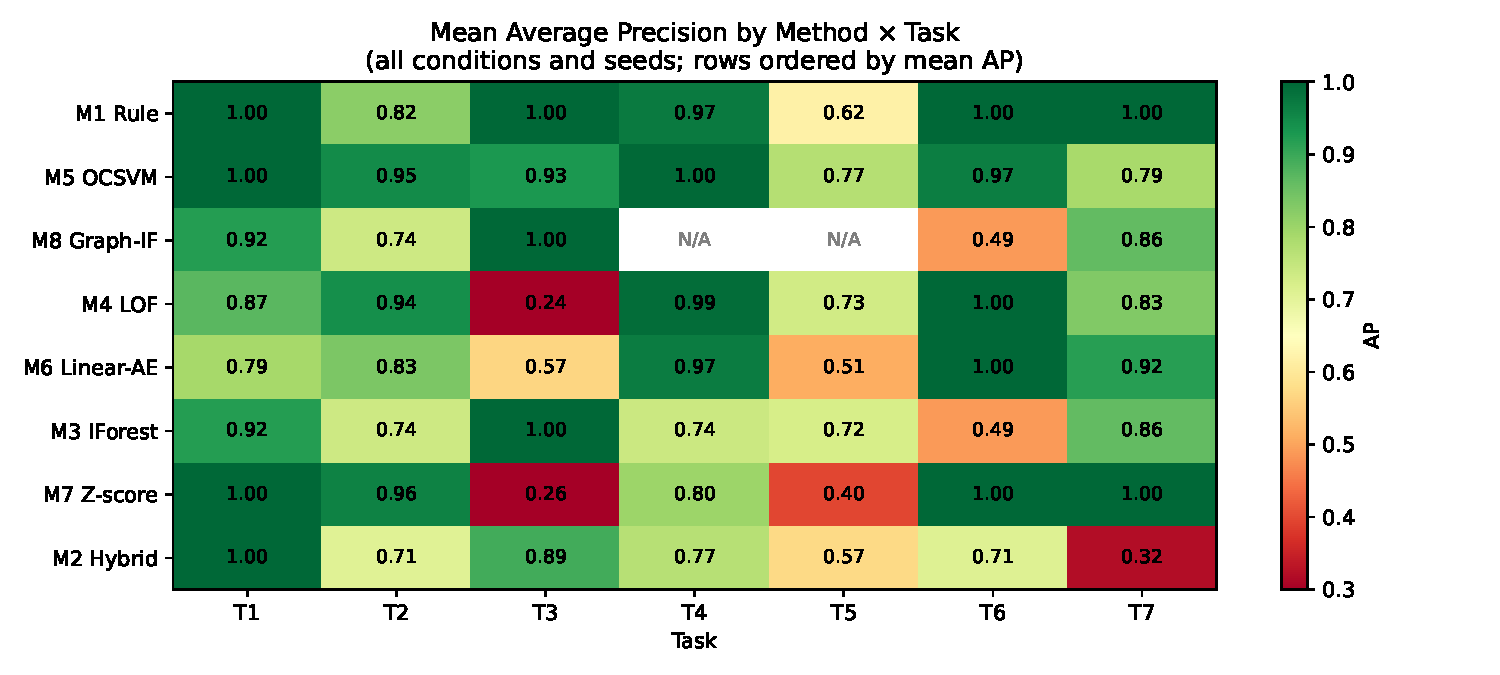
\includegraphics[width=\columnwidth]{figures/fig1_ap_heatmap}
  \caption{Mean AP by method and task, averaged across all five telemetry conditions and three seeds. Darker cells indicate higher AP. M1 (rule baseline) dominates on 5 of 7 tasks; M5 (OCSVM) and M7 (temporal z-score) achieve the highest ML AP on T2 and T5 respectively.}
  \label{fig:ap_heatmap}
\end{figure}

\subsection{Where ML Adds Value}

ML consistently outperforms the rule baseline on two tasks
(Table~\ref{tab:ml_gain}; Figure~\ref{fig:ml_gain} shows full per-condition breakdowns).

\textbf{T2 --- Group Membership Drift.} The rule baseline achieves AP~=~0.766
(C-BASE). Three ML methods consistently improve on this: M7 temporal z-score
(AP~=~0.951, $\Delta$AP~=~$+$0.185), M5 OCSVM (AP~=~0.913, $+$0.147), and M4 LOF
(AP~=~0.890, $+$0.124). Group-membership anomalies involve multi-dimensional
population-level deviations that temporal z-score and kernel-based methods capture
more precisely than fixed-threshold rules.

\textbf{T5 --- Patch--Vulnerability Hygiene.} Rule AP~=~0.458 (C-BASE). Best ML:
M5 OCSVM (AP~=~0.668, $\Delta$AP~=~$+$0.210). T5 combines multiple vulnerability
signals (CVSS score, KEV exposure, remediation latency, days open) in ways that
benefit from learned combinations. Absolute AP remains low across all methods,
indicating genuine task difficulty.

\begin{table}[t]
\centering
\caption{Configurations where ML consistently outperforms rule
  baseline (B/S = BASE\,+\,STALE conditions combined).}
\label{tab:ml_gain}
\footnotesize
\setlength{\tabcolsep}{4pt}
\begin{tabular}{@{}llrrrr@{}}
\toprule
Task & Method & Rule AP & ML AP & $\Delta$AP & Cond. \\
\midrule
T2 & M7 Z-score & 0.766 & 0.951 & $+$\textbf{0.185} & B/S \\
T2 & M4 LOF     & 0.855 & 0.975 & $+$\textbf{0.120} & C-MISS \\
T5 & M5 OCSVM   & 0.458 & 0.668 & $+$\textbf{0.210} & B/S \\
T5 & M5 OCSVM   & 0.726 & 0.837 & $+$\textbf{0.111} & C-MISS \\
\bottomrule
\end{tabular}
\end{table}

\begin{figure*}[t]
  \centering
  
\includegraphics[width=\textwidth]{figures/fig4_t2_t5_ml_gain}
  \caption{T2 (group membership drift) and T5 (patch/vulnerability hygiene) AP by method and condition. These are the only two tasks where ML consistently outperforms the rule baseline by the pre-registered $\Delta \geq 0.05$ threshold in $\geq$2/3 seeds. M7 (temporal z-score) achieves the best AP on T2 (+0.185 over rule); M5 (OCSVM) achieves the best AP on T5 (+0.210 over rule).}
  \label{fig:ml_gain}
\end{figure*}

\subsection{Telemetry Condition Effects}

Figure~\ref{fig:ap_by_condition} plots the AP distributions by condition.
C-STALE produces the lowest mean AP (0.741 vs.\ C-BASE 0.772, $\Delta$~=~$-$0.031).
The largest staleness degradation is T3 (endpoint--identity correlation): AP drops
from 0.782 (C-BASE) to 0.613 (C-STALE, $\Delta$~=~$-$0.168). T3 combines
identity-side and endpoint-side features; staleness in either degrades the joint
signal, making T3 the strongest argument for staleness-aware detection methods.

Table~\ref{tab:conditions} summarizes mean AP by condition.
C-FRESH, C-MISS, and C-UNSUP show higher mean AP than C-BASE (0.856, 0.845, 0.844
respectively). The primary contributor is T5, which gains $+$0.238 AP under C-FRESH.
Fresh telemetry improves patch compliance scores and KEV exposure count reliability,
making underlying feature signals more discriminating---a data-quality effect, not a
freshness-flag artifact.

\begin{table}[t]
\centering
\caption{Mean AP by telemetry condition (all methods and tasks).}
\label{tab:conditions}
\small
\begin{tabular}{@{}lrrl@{}}
\toprule
Condition & Mean AP & $\Delta$ vs C-BASE & Primary driver \\
\midrule
C-FRESH & 0.856 & $+$0.084 & T5 $+$0.238, T1 $+$0.101 \\
C-MISS  & 0.845 & $+$0.073 & Similar to C-FRESH \\
C-UNSUP & 0.844 & $+$0.072 & Labels withheld only \\
C-BASE  & 0.772 & ---       & Reference \\
C-STALE & 0.741 & $-$0.031 & T3 $-$0.168 \\
\bottomrule
\end{tabular}
\end{table}

\begin{figure}[t]
  \centering
  
\includegraphics[width=\columnwidth]{figures/fig3_ap_by_condition}
  \caption{AP distribution by telemetry condition across all methods and tasks. C-STALE produces the lowest median AP; C-FRESH and C-MISS elevate performance on tasks where telemetry freshness is discriminative (primarily T1 and T5).}
  \label{fig:ap_by_condition}
\end{figure}

\subsection{Failure-Flag Analysis}

Figure~\ref{fig:failure_heatmap} shows the per-(method, task) failure-flag heatmap.
M8 (graph-augmented IF) is failure-flagged on all 75 applicable configurations
(100\%). The largest M8 deficit is T6 (dormant account reactivation): M8 AP~=~0.490
vs.\ M1 AP~=~1.000. Bipartite user-group graph features capture structural position
but not temporal account state, which is the primary T6 signal. M5 (OCSVM) has the
lowest failure rate (69.5\%) and succeeds on T2 and T5. M2 (hybrid scorer) has the
highest failure rate among non-graph methods (96.2\%), indicating that its
fixed-weight combination is not well-calibrated across the heterogeneous task set.

\begin{figure}[t]
  \centering
  
\includegraphics[width=\columnwidth]{figures/fig2_failure_heatmap}
  \caption{Failure-flag fraction per (method, task) cell across all conditions and seeds. Red = high failure rate ($\geq$80\%); blue = low failure rate. M8 (graph-IF) is uniformly red (100\% failure rate). M5 (OCSVM) achieves the lowest failure rate (69.5\%).}
  \label{fig:failure_heatmap}
\end{figure}

T7 (escalation drift) exhibits a ceiling effect: with only 2 anomalous entities per
dataset instance (imbalance $\approx$1:500), all methods achieve AP~=~1.000 because
every method places those entities above the majority.

% =====================================================================
\section{Discussion and Limitations}
\label{sec:discussion}

\textbf{Interpretation.} The 86.2\% failure rate is not a finding against ML in
security operations broadly. It is a finding about unsupervised ML vs.\ structured
rule baselines on \emph{synthetic, class-imbalanced tabular anomaly detection} in
the hygiene domain. Real operational environments involve noisier data, absent
labels, and anomaly presentations more overlapping with normal behavior. The
synthetic benchmark tests whether methods can detect structurally clear anomalies;
the two tasks where ML adds value (T2, T5) are those involving multi-signal
combinations that benefit from learned representations.

\textbf{Limitations.} (1) All telemetry is synthetic; performance on real
operational data will differ. (2) M6 is implemented as PCA-based linear
reconstruction error, not a neural autoencoder; M8 uses networkx features rather
than a full deep graph autoencoder \cite{ding2019dominant}. Both are disclosed
approximations. (3) Population scale ($n$=1,000) is smaller than most public-sector
environments. (4) Feature extractors encode domain knowledge; methods exploiting
these features appear better. (5) No score calibration is performed; calibration is
excluded by design. (6) AD group-size distributions lack a peer-reviewed prior source.

\textbf{Practical implications.}
\hb supports three practitioner decisions. First, for tasks where rule baselines
already achieve AP~$\geq$~0.90 (T1, T4, T6), practitioners should weigh the
maintenance overhead of ML against minimal detection gain: \hb provides no evidence
that ML justifies that overhead on synthetic structured data. Second, for T2 and T5,
ML (OCSVM, temporal z-score, LOF) provides measurable lift over rules, motivating
investment in supervised or semi-supervised variants if labels become available.
Third, the C-STALE results quantify the detection cost of stale data pipelines: the
$-$0.168 AP drop on T3 under C-STALE is a conservative lower bound on what SOCs risk
when telemetry ingestion lags.

\textbf{Future work.}
Planned extensions include: (i) $n$=10,000 large-scale instances to test statistical
power under lower imbalance ratios; (ii) supervised baselines (gradient-boosted
trees) to bound the label-value ceiling; (iii) full neural autoencoder (M6) and
DOMINANT-style deep graph autoencoder (M8) once a GPU environment is available;
(iv) PoC-label and ExploitDB-enriched vulnerability records to make T5 harder;
(v) catalog-perturbation sensitivity sweeps on the structural priors (DBIR patch lag,
NVD severity) to characterize robustness to prior misspecification.

% =====================================================================
\section{Conclusion}
\label{sec:conclusion}

We introduced \hb, a reproducible synthetic benchmark for cyber-hygiene anomaly
detection spanning seven tasks, twelve anomaly classes, and eleven entity/event
tables generated from a fully open, seeded pipeline grounded in public structural
priors (NIST NVD, Verizon DBIR 2026, CISA BOD 23-01 \cite{cisa_bod2301_2022}).
An 810-run evaluation of eight methods under five telemetry conditions, using a
pre-registered failure protocol, finds that simple rule baselines perform at least
as well as unsupervised ML on \textbf{86.2\%} of (condition, task, method)
configurations. ML adds consistent value on group membership drift (T2, $+$0.185 AP,
M7 temporal z-score) and patch-vulnerability hygiene (T5, $+$0.210 AP, M5 OCSVM).
M8 (graph-IF) is failure-flagged on all 75 applicable configurations. Telemetry
staleness consistently degrades performance; T3 (endpoint--identity correlation) is
the most sensitive task ($-$0.168 AP under C-STALE), quantifying the detection cost
of stale data pipelines.

These results motivate three benchmark-practice changes: (1) task-stratified
reporting over macro-averaged summaries; (2) negative-result protocols as
first-class contributions; (3) telemetry freshness as a mandatory evaluation axis.

\hb v0.1 (generator, datasets, evaluation harness) is openly released at
\url{https://doi.org/10.5281/zenodo.20438401}.

% =====================================================================
\balance
\bibliographystyle{IEEEtran}
\bibliography{references}

\end{document}
